\section{Evaluation} \label{sec:evaluation}
%[\textbf{Todo: list experimental evaluation steps.}]

\begin{table}
    \centering
    \begin{tabular}{c|c|c}
        \toprule 
    Method  & Average Quality & Average Volume \\
    \midrule 
    \textit{M0} & $0.0879\pm0.0290$ & $10$ \\
    \textit{M1} & $0.3673\pm0.1569$ & $10$ \\
    \textit{M2} & $0.4097\pm0.1313$ & $9$ \\
    \textit{M3} & $0.5295\pm0.0816$ & $6$ \\
    \bottomrule
    \end{tabular}
    \caption{Average quality ($G$) and volume of teams (\#$T$) shown \textit{per} researcher ($r_j$) at USC. This was done for each method $M_i$, across 434 RFPs and 200 researchers. For average quality, we report the mean and standard deviation, denoted as \texttt{mean$\pm$STD}.} \label{tab:volume_quality}
\end{table}

\subsection{Computational Evaluation of Output}
\subsubsection{Quality vs. Volume of Teams.}
%We use a $k$-fold cross validation ($k=5$) to evaluate each of the four methods, where the datasets are divided into 5 equal subsets and, in each of the five runs, four subsets are used for training and the remaining one for testing.
%\likitha{Talk about the results from ppt and link to those graphs in Ultra-github.}

For each method, we assess the quality (goodness) and volume (size) of each teaming suggestion that every researcher $r_j$ receives per every call for proposal $c_i$. Our experiments iterate across a dataset of 434 RFPs and 200 researchers. For each call, every researcher has a maximum cutoff of 10 teams. For each method, we then find the average goodness ($G$) of teams $(T)$ a researcher $r_j$ has been recommended.
%\footnote{Additional details about data, experiments, and graphical results are at \cite{ultra-resources}.}. 
The more advanced the method, the better teams a researcher receives. We observe another unique trade-off as a result, where teams formed algorithmically led to an increased precision and quality, and a notable decrease in quantity. \textit{M0}, random team formation, showed poor quality in results with an average goodness of only $0.0879,$ despite the number of teams being abundantly available. \textit{M3}, on the other hand, shows a decrease in the number of teaming choices available for a researcher, but a visible increase in quality, compared to the average goodness for \textit{M0}.
Table~\ref{tab:volume_quality} shows the overall results. 

\subsection{Human Evaluation of Output} 

We deployed our tool at a college-wide level and requested participation from faculty members. This research study has been IRB-approved by our university (IRB\#~Pro00127449) and reflects an observational (unmonitored) qualitative analysis, where we make the tool publicly available and give participants a demo of its usage but do not actively control their actions. This helps us receive many responses quickly and at a low cost, albeit not without its own limitations. For instance, it does not require users to explore all use cases and methods. Therefore, we only make inferences from data that is recorded and do not draw any from those that are left out. As a possible future work, we can perform a controlled qualitative analysis, where we request participants to come to a designated lab, try every pathway, and give feedback. This will then enable us to answer how a user compared the effectiveness of each method on the same example. 

\begin{table}[ht]
{\renewcommand\arraystretch{1.25}
{\begin{tabular}{l|l|l} \hline
& \multicolumn{2}{l}{Qualitative Results} \\ \hline
Comments & \multicolumn{2}{p{6cm}}{1. \raggedright \textit{``This is incredible and has a lot of potential. Can't wait for this to be in real time!"}} \\ 
 & \multicolumn{2}{p{6cm}}{2. \raggedright \textit{``Very well thought out! Great resource to the university"}} \\ 
 & \multicolumn{2}{p{6cm}}{3. \raggedright \textit{``Lots of new people to choose from here! Great work!"}} \\ 
 & \multicolumn{2}{p{6cm}}{4. \raggedright \textit{``Very useful tool  overall, I could see the practical usage of this work!"}} \\ 
 & \multicolumn{2}{p{6cm}}{5. \raggedright \textit{``Would love an explanation for all of your methods used!!"}} \\ 
 \hline
Feedback & \multicolumn{2}{p{6cm}}{1. \raggedright \textit{``Seeing many team pitches here from interdisciplinary domains. Can we choose from say, two, settings where we may choose to work with those from a similar domain or a different one? And how so is the overall goodness score calculated?"}} \\ 
 & \multicolumn{2}{p{6cm}}{2. \raggedright \textit{``A search bar would be great for this one, not just a dropdown!"}} \\ 
 & \multicolumn{2}{p{6cm}}{3. \raggedright \textit{``In addition to the proposal, can we also add research interest as a user-given input? As a merging of the second and third use cases"}} \\ 
 & \multicolumn{2}{p{6cm}}{4. \raggedright \textit{``can we build our own teams for a grant?"}} \\ 
 
\hline
\end{tabular}}}
\caption{A sample of the comments as well as feedback for improvement received from the human study.} \label{tab:comments_feedback}
\end{table}

We received a total of 212 responses. Regarding relevancy of outputs, 157 answers were rated as \textit{very relevant} and 34 as \textit{somewhat relevant}, summing to 90.09\% of all responses. Similarly, in terms of tool utility satisfaction, 172 answers responded with \textit{very useful} and 35 with \textit{somewhat useful}, totaling 97.64\% of all responses. Figure~\ref{fig:sankey_human_study} shows a more quantitative breakdown of the responses and Table~\ref{tab:comments_feedback} highlights a few comments and feedback we received. 

\label{subsec:humanstudy}
\begin{figure*}
    \centering
    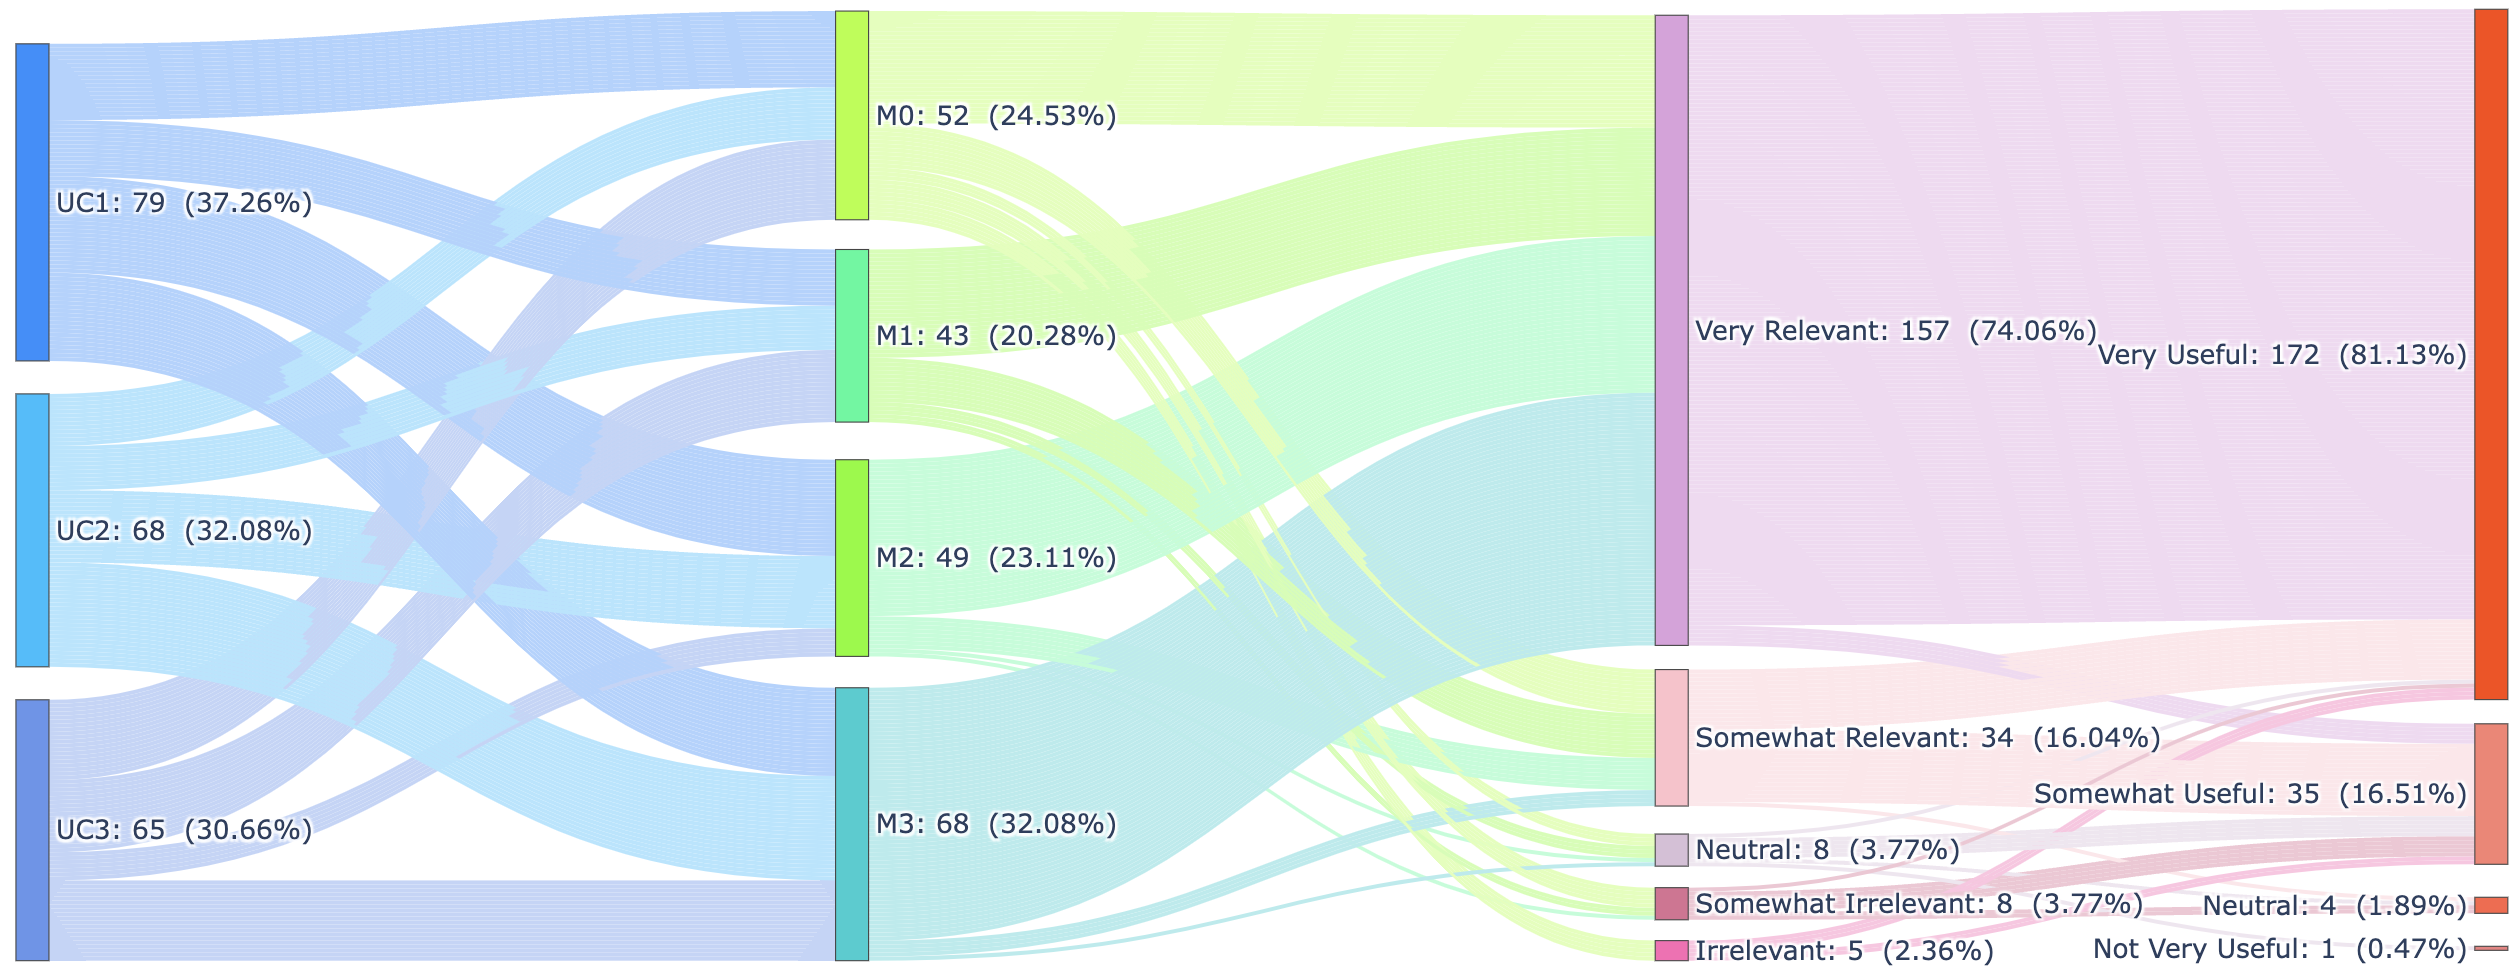
\includegraphics[width=0.85\textwidth]{figures/ultra_human_study_sankey_enlarged.png}
    \caption{Sankey breakdown of the 212 responses we received from our human study. It shows four categories of nodes: (1)~use cases, (2)~methods, (3)~scale of relevancy, and (4)~scale of usefulness. Each line maps a connection from node type to another, showing the flow of interaction that users had with ULTRA. }
    \label{fig:sankey_human_study}
\end{figure*}


We observe two repeated patterns of responses regarding \textit{M0}: (1) Teaming choices that were rated as \textit{`somewhat irrelevant'} or \textit{`irrelevant'}, yet still \textit{`very useful'}, and (2) teaming choices that were rated as \textit{`very relevant'}, despite the irrelevancy in the results. Upon analyzing the comments, some mentioned that \textit{M0} could regardless be useful in working with new colleagues from other departments and \textit{`expand new connections'} as a result. Furthermore, we have only requested users to judge the \textit{usability} and \textit{functionality} of our tool, not immediate applicability. They may also be unaware of each candidate member's skill set, which impedes on their ability to accurately quantify a team's success. Due to that, there is a need and role of AI in teaming, as reflected in comments as well. We also factor this intuition into the interpretation of results. 

